% ─────────────────────────────────────────────────────────────────
\section{Dataset: SHREC\,25 Protein Surfaces}
\label{sec:dataset}
% ─────────────────────────────────────────────────────────────────

\subsection{Overview}

The SHREC\,25 Protein Surface Classification dataset consists of triangulated
surface meshes extracted from protein structures in the Protein Data Bank.
Each mesh is annotated with a SCOP fold class label.
Table~\ref{tab:dataset_stats} summarises the key statistics.

\begin{table}[h]
  \centering
  \caption{SHREC\,25 dataset statistics.}
  \label{tab:dataset_stats}
  \begin{tabular}{lrr}
    \toprule
    \textbf{Property} & \textbf{Value} & \textbf{Notes} \\
    \midrule
    Total classes          & 99  & SCOP fold families \\
    Training proteins      & 9\,244  & 97 classes represented \\
    Test proteins          & 2\,311  & 88 classes represented \\
    Classes with 0 test    & 9   & excluded from macro-F1 \\
    Classes with 1 test    & 6   & near-zero contribution \\
    \midrule
    Avg.\ vertices / mesh  & $\approx$10\,676 & surface triangulation \\
    Scalar fields          & 2   & Potential, NormalPotential \\
    \midrule
    Most frequent class    & 2\,054 train / 514 test & class\,8 \\
    Least frequent class   & 2 train & class\,26 \\
    \textbf{Imbalance ratio} & \textbf{1\,027$\times$} & train set \\
    \bottomrule
  \end{tabular}
\end{table}

\subsection{Class Imbalance}

Figure~\ref{fig:class_dist} shows the sorted training count per class on a
log scale, together with the cumulative distribution function.
The distribution is highly long-tailed: roughly 42\% of classes have fewer
than 10 training examples, and the top class alone accounts for 22\% of all
training proteins.
This severe imbalance drives the choice of inverse-square-root class
weighting in the cross-entropy loss (Section~\ref{sec:training}).

\begin{figure}[h]
  \centering
  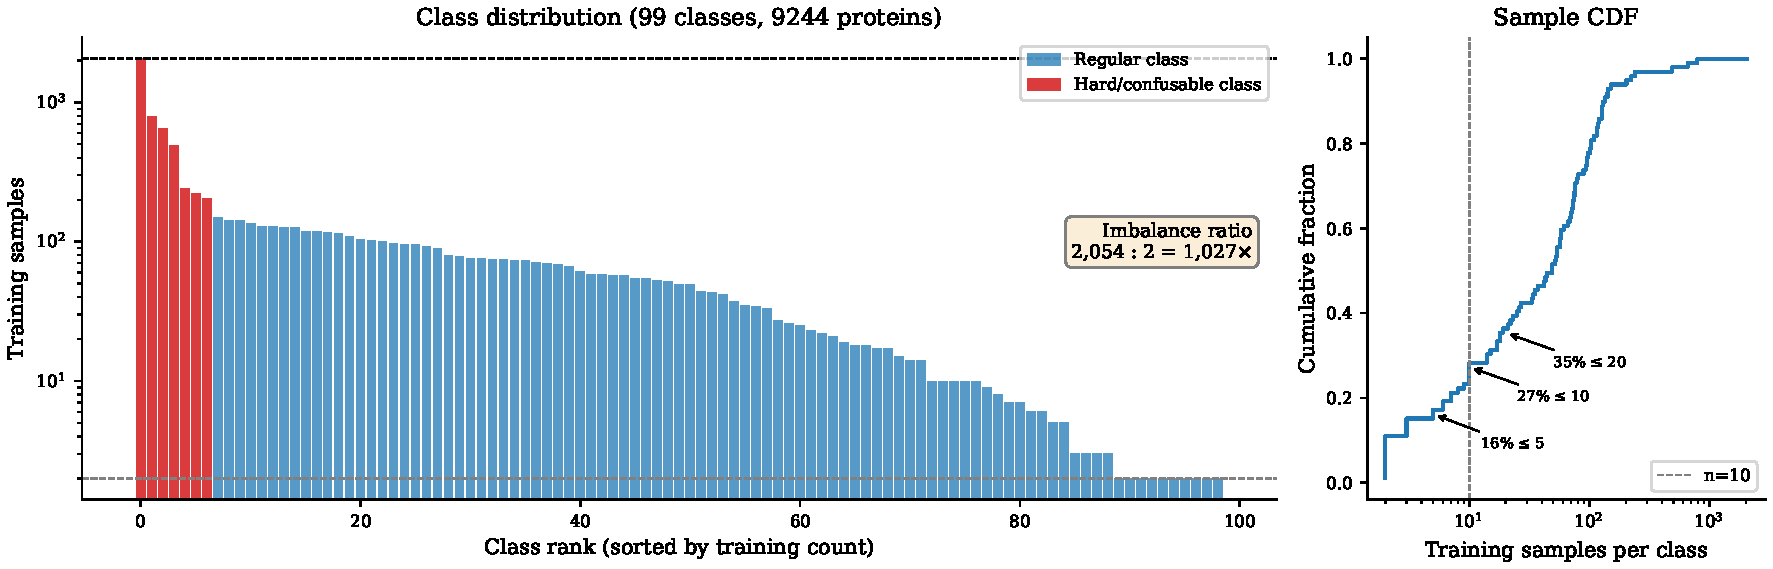
\includegraphics[width=\linewidth]{figures/class_distribution.pdf}
  \caption{Class distribution (99 classes, 9\,244 training proteins).
           Left: sorted sample count per class on log scale; orange bars
           highlight the hard/confusable classes studied in depth.
           Right: cumulative distribution of sample counts per class.}
  \label{fig:class_dist}
\end{figure}

\subsection{Per-mesh Features}

Each VTK surface mesh provides:
\begin{itemize}
  \item \textbf{Vertex positions} $(x, y, z)$ --- the three-dimensional
        coordinates of the triangulation vertices.
  \item \textbf{Surface normals} $(n_x, n_y, n_z)$ --- unit normals
        estimated from the local triangulation.
  \item \textbf{Electrostatic potential} (\textit{Potential}) --- a scalar
        field representing the Coulombic potential at each vertex, computed
        from atomic partial charges.  Values span a wide dynamic range
        (typically $-$50 to $+$50\,kcal/mol/e).
  \item \textbf{Normal potential} (\textit{NormalPotential}) --- the normal
        component of the potential gradient; a secondary scalar field that
        characterises surface charge concentration.
\end{itemize}

All scalars are z-scored at training time and clamped to $[\!-5, 5\!]$
to suppress outliers before they are fed to the GNN (Section~\ref{sec:pipeline}).

\subsection{Hard and Confusable Class Pairs}

A statistical separability study (Section~\ref{sec:analysis}) identifies three
pairs of classes that are consistently confused across all models and feature
configurations:

\begin{center}
  \begin{tabular}{cccc}
    \toprule
    \textbf{Pair} & \textbf{SVM bal.\ acc.\ (graph)} & \textbf{SVM bal.\ acc.\ (VTK)} & \textbf{Status} \\
    \midrule
    (61, 90) & 0.543 & 0.563 & Near-inseparable \\
    (70, 56) & 0.573 & 0.598 & Partially separable \\
    (86, 14) & 0.665 & 0.699 & Better separated \\
    \bottomrule
  \end{tabular}
\end{center}

These pairs share similar overall electrostatic profiles but belong to
different SCOP families. The classification errors on these pairs are
effectively irreducible with the current feature set.
